\documentclass[12pt,twocolumn]{article}

\usepackage[a4paper,margin=0.75in,top=1in,bottom=1in,headheight=14pt]{geometry}
\usepackage[T1]{fontenc}
\usepackage{mathptmx}
\usepackage{fancyhdr}
\usepackage{lastpage}
\usepackage{booktabs}
\usepackage{array}
\usepackage{tabularx}
\usepackage{float}
\usepackage{graphicx}
\usepackage{amsmath}
\usepackage{enumitem}
\usepackage{tikz}
\usetikzlibrary{shapes.geometric,arrows.meta,positioning,calc,fit,
                 backgrounds,decorations.pathreplacing,patterns}
\usepackage{xcolor}
\usepackage{setspace}
\usepackage{titlesec}
\usepackage{caption}
\usepackage{pifont}
\newcommand{\cmark}{\ding{51}}
\usepackage[style=apa,natbib=true,backend=biber,uniquename=false,uniquelist=false]{biblatex}
\addbibresource{references.bib}
\usepackage{hyperref}
\hypersetup{
  pdftitle={Self-Consistent Error Detection in LLMs},
  pdfauthor={Simranjeet Singh},
  colorlinks=true,
  linkcolor=blue!60!black,
  citecolor=blue!60!black,
  urlcolor=blue!60!black,
}

\definecolor{ceRed}{HTML}{E74C3C}
\definecolor{ieOrange}{HTML}{F39C12}
\definecolor{rcGreen}{HTML}{27AE60}
\definecolor{fcYellow}{HTML}{F1C40F}
\definecolor{naGray}{HTML}{95A5A6}
\definecolor{phase1Blue}{HTML}{3498DB}
\definecolor{phase2Green}{HTML}{2ECC71}
\definecolor{wbPurple}{HTML}{9B59B6}
\definecolor{lightbg}{HTML}{F8F9FA}

\singlespacing
\setlength{\parskip}{2pt}
\setlength{\parindent}{0pt}

\titleformat{\section}{\normalfont\large\bfseries}{\thesection.}{0.5em}{}
\titleformat{\subsection}{\normalfont\normalsize\bfseries}{\thesubsection}{0.5em}{}
\titlespacing*{\section}{0pt}{8pt}{2pt}
\titlespacing*{\subsection}{0pt}{6pt}{1pt}
\titlespacing*{\subsubsection}{0pt}{4pt}{1pt}

\pagestyle{fancy}
\fancyhf{}
\fancyhead[L]{\small Page \thepage\ of \pageref{LastPage}}
\fancyhead[R]{\small Singh, Simranjeet}
\renewcommand{\headrulewidth}{0.4pt}

\captionsetup{font=small,labelfont=bf,skip=4pt}

\begin{document}

% ====================================================================
% TITLE PAGE (full width)
% ====================================================================
\twocolumn[
\begin{@twocolumnfalse}
\begin{center}
\vspace*{1cm}
{\LARGE\bfseries Self-Consistent Error Detection in Closed and Open\\
Large Language Models: A Black-Box and White-Box\\Comparative Study}

\vspace{0.6cm}
{\large Final Report -- Undergraduate Thesis}

\vspace{0.8cm}
{\large Simranjeet Singh}

\vspace{0.3cm}
Department of Computer Science, Western University

\vspace{0.3cm}
Thesis Supervisor: Prof.\ Lucian Ilie, Dept.\ of Computer Science

\vspace{0.1cm}
Course Coordinator: Prof.\ Nazim Madhavji, Dept.\ of Computer Science

\vspace{0.3cm}
March 2026

\vspace{0.8cm}
\end{center}
\end{@twocolumnfalse}
]

% ====================================================================
% GLOSSARY
% ====================================================================
\section*{Glossary}

\begin{description}[style=nextline,leftmargin=1.8cm,font=\normalfont\bfseries,nosep,itemsep=2pt]
\item[LLM] Large Language Model: a neural network trained on large text
      corpora to generate human-like text.
\item[CE] Self-Consistent Error: a question the model answers incorrectly
      with the same incorrect answer across all stochastic samples.
\item[IE] Inconsistent Error: a question the model answers incorrectly
      with varying answers across stochastic samples.
\item[NLI] Natural Language Inference: a classification task determining
      whether a hypothesis is entailed by, contradicts, or is neutral to a
      premise.
\item[AUROC] Area Under the Receiver Operating Characteristic curve: a
      metric measuring classifier discrimination ability.
\item[FFN] Feedforward Neural Network: a probe architecture used for
      hidden-state classification.
\item[MoE] Mixture-of-Experts: an architecture activating only a subset
      of parameters per input.
\item[HPC] High-Performance Computing: cluster computing environment
      (Nibi cluster used in this work).
\item[TruthfulQA] A benchmark of 817 questions designed to elicit
      imitative falsehoods from language models \citep{lin2022truthfulqa}.
\end{description}

% ====================================================================
% STRUCTURED ABSTRACT
% ====================================================================
\section*{Structured Abstract}

\textbf{Context.}
Large Language Models (LLMs) sometimes produce confident but incorrect
answers, a phenomenon known as hallucination. A particularly dangerous
subtype is the \emph{self-consistent error} (CE), in which the model
repeats the same incorrect answer across independent samples, rendering
output-based consistency detectors ineffective \citep{tan2025consistent}.

\textbf{Objective.}
This thesis investigates three questions: (1)~how prevalent are CEs
across both closed-source and open-weight frontier LLMs, (2)~whether
cross-model hidden-state probes using small proxy encoders can detect
CEs in API-only models, and (3)~whether CEs decrease as model
families evolve.

\textbf{Method.}
A two-phase black-box pipeline evaluated six models (four
closed-source APIs, two open-weight) on 807 TruthfulQA questions
(4,842 rows). Correctness was judged by a three-model ensemble;
semantic equivalence used hybrid NLI with LLM fallback. A white-box
cross-model probe, adapted from \citet{tan2025consistent}, was
extended with small proxy encoders (3B--4B parameters) to enable
hidden-state analysis for all six targets including closed-source
APIs. A version-evolution study tracked CE rates over four
generations in three families (Grok, Llama, Qwen; 12~models,
9,684~rows).

\textbf{Results.}
At equivalence threshold $t{=}1.0$ (all stochastic samples must
match the greedy answer), 42.1\% of incorrect answers were
self-consistent errors. Proxy-based probes achieved CE AUROC of
0.85--1.00 (mean 0.93) across all six targets. In the evolution
study, only the Grok family showed monotonic CE reduction (17.7\%
$\to$~0.5\%, every step $p < 0.001$); Llama and Qwen exhibited
non-monotonic patterns.

\textbf{Conclusion.}
Self-consistent errors are prevalent across both closed-source and
open-weight models, and are amenable to proxy-based hidden-state
probing even when the target's own representations are inaccessible.
CE reduction across generations is achievable but not guaranteed,
highlighting the need for explicit CE tracking in model development.

% ====================================================================
% TABLE OF CONTENTS
% ====================================================================
\tableofcontents
\clearpage

% ====================================================================
% 1. INTRODUCTION
% ====================================================================
\section{Introduction}
\label{sec:intro}

Large Language Models (LLMs) are now widely used for information
retrieval, code generation, and decision support
\citep{huang2025survey}. They are increasingly deployed in
high-stakes domains such as healthcare, legal research, and finance,
where a confidently stated falsehood can cause real harm. Yet LLMs
regularly produce factually incorrect outputs that appear
plausible, a phenomenon known as \emph{hallucination}
\citep{ji2023hallucination}. Not all hallucinations carry the same
risk. When an LLM produces different incorrect answers each time it
is queried, the inconsistency itself acts as a warning signal:
users or automated systems can detect the variation and flag the
answer for review. However, when the model repeats the \emph{same}
incorrect answer across independent samples, no such signal exists.
The error becomes undetectable by any method that relies on output
variation.

\citet{tan2025consistent} formalised this distinction by defining a
\textbf{self-consistent error~(CE)}: a question for which the greedy
answer is incorrect and all stochastic samples are semantically
equivalent to that greedy answer. They showed that existing
hallucination detectors, particularly those based on output
consistency such as sampling-and-voting
\citep{wang2023selfconsistency} perform at or below chance on CEs
\citep{tan2025consistent}.
To address this, they proposed a \textbf{cross-model hidden-state
probe} that uses internal representations from a second ``verifier''
model to detect errors that the response model's own outputs
conceal. However, their evaluation was limited to open-source models
on TriviaQA and SciQ. It remained unclear whether the same CE
patterns exist in closed-source API models such as Claude, GPT, and
Grok, and whether cross-model probing can work when the target
model's hidden states are inaccessible.

This thesis addresses three research questions:
\begin{description}[nosep,leftmargin=0.5cm,font=\normalfont\bfseries]
\item[RQ1:] How prevalent are self-consistent errors across both
  closed-source and open-weight frontier LLMs?
\item[RQ2:] Can cross-model hidden-state probes, using small proxy
  encoders, detect CEs in API-only models whose hidden states are
  inaccessible?
\item[RQ3:] Do CEs decrease as model families evolve over successive
  generations?
\end{description}

These questions are investigated along three corresponding axes:
\begin{enumerate}[nosep]
\item \textbf{Black-box measurement (O1).} A two-phase pipeline
      measured CE rates across six frontier LLMs, including both
      closed-source APIs (Claude Opus~4.6, GPT-5.2, Grok~4,
      DeepSeek~V3.2) and open-weight models (Qwen3 Next~80B,
      Llama~4 Maverick), on 807 TruthfulQA questions
      \citep{lin2022truthfulqa}, producing 4,842 evaluated rows.
      TruthfulQA was chosen because it provides ground-truth
      reference answers, enabling reliable automated CE labelling.
\item \textbf{White-box detection (O2).} The cross-model probe of
      \citet{tan2025consistent} was adapted and extended: instead of
      requiring the target model's own hidden states, two small
      open-weight models (3B and 4B parameters) were used as
      \emph{proxy encoders}, enabling hidden-state analysis for all
      six targets including the four closed-source APIs. CE AUROC
      ranged from 0.85 to 1.00.
\item \textbf{Version-evolution study (O3).} CE rates were tracked
      across four consecutive generations in three model families
      (Grok, Llama, Qwen), covering 12~models and 9,684~rows.
\end{enumerate}

The key findings are: (a)~42.1\% of incorrect answers are
self-consistent at equivalence threshold $t{=}1.0$ (i.e., all ten
stochastic samples match the greedy answer), (b)~proxy-based
cross-model probes achieve strong CE detection (AUROC 0.85--1.00)
across all six targets, including closed-source APIs, and (c)~only
the Grok family exhibited monotonic CE reduction across generations
(17.7\%~$\to$~0.5\%), while Llama and Qwen showed no consistent
improvement.

This work is the first to combine black-box CE measurement on
closed-source frontier models, proxy-based cross-model probing for
API-only targets, and a longitudinal evolution study within a single
framework on TruthfulQA.

The remainder of this report is organised as follows.
Section~\ref{sec:background} reviews related work and identifies the
research gap. Section~\ref{sec:goals} states the research goal and
objectives. Section~\ref{sec:method} describes the methodology.
Section~\ref{sec:results} presents results.
Section~\ref{sec:discussion} discusses threats, implications, and
limitations. Section~\ref{sec:conclusions} gives conclusions, and
Section~\ref{sec:future} outlines future work.

% ====================================================================
% 2. BACKGROUND AND RELATED WORK
% ====================================================================
\section{Background and Related Work}
\label{sec:background}

\subsection{LLM Hallucination}
\label{sec:bg-hallucination}

Hallucination in natural language generation refers to content that is
fluent and confident but factually unsupported or contradicted by
world knowledge \citep{ji2023hallucination}. \citet{huang2025survey}
classify hallucinations into
\emph{factuality hallucinations} (contradicting established facts)
and \emph{faithfulness hallucinations} (diverging from a provided
source). This thesis focuses on factuality hallucinations in a
closed-book question-answering setting, where no external source is
provided and the model must rely on its parametric knowledge.

Hallucination frequency alone does not capture the full risk
profile. A model that qualifies its response (``I am not sure, but
possibly\ldots'') poses less risk than one that states a falsehood
without hedging. This distinction between \emph{confident} and
\emph{uncertain} errors motivates the self-consistent error
framework described in Section~\ref{sec:bg-ce}
\citep{tan2025consistent}.

\subsection{The TruthfulQA Benchmark}
\label{sec:bg-truthfulqa}

TruthfulQA \citep{lin2022truthfulqa} is a benchmark of 817 questions
across 38 categories designed to elicit imitative falsehoods:
incorrect answers that models produce because they reflect common
human misconceptions. Categories include health, law, conspiracies,
and fiction. For example, the health category contains questions
about medical myths (e.g., ``Can spicy food give you ulcers?''),
while the misconceptions category tests persistent folk beliefs
(e.g., ``What happens if you swallow gum?''). Unlike
general-knowledge benchmarks such as TriviaQA or Natural Questions,
TruthfulQA targets questions where popular but incorrect beliefs
exist, making it well suited for studying confident misinformation.
Each question provides a best answer and lists of acceptable correct
and incorrect answers, enabling automated evaluation. Of the
original 817 questions, this thesis uses 807 after removing 10 that
could not be reliably judged by the automated pipeline.

\subsection{Self-Consistent Errors}
\label{sec:bg-ce}

\citet{tan2025consistent} introduced the formal
concept of a self-consistent error. Given a question~$q$, let $a_g$
be the model's greedy (deterministic) answer and let
$\{a_1, \ldots, a_n\}$ be $n$ stochastic samples generated at
temperature $T > 0$. The response is a CE if $a_g$ is incorrect and
all $a_i$ are semantically equivalent to $a_g$.

To illustrate, consider the TruthfulQA question \emph{``What happens
if you swallow gum?''} The correct answer is that gum passes through
the digestive system. A model exhibiting a CE would answer \emph{``It
stays in your stomach for seven years''} as its greedy response, and
all ten stochastic samples would produce semantically equivalent
paraphrases of the same misconception. The model is incorrect, confident,
and produces no variation. An output-consistency detector would
observe perfect agreement and incorrectly classify the answer as
reliable \citep{lin2022truthfulqa, tan2025consistent}.

Their study made two empirical contributions relevant to this
thesis. First, CEs do \emph{not} decrease with model scale: unlike
inconsistent errors, which tend to diminish as models grow larger,
CEs remain stable or increase. Second, existing hallucination
detectors (including consistency-based methods, uncertainty
estimators, and some internal-state probes) degrade substantially
when evaluated on CEs. Consistency-based detectors are the most
affected because CEs produce uniformly similar outputs and
therefore exhibit low output variance. The same property that makes
CEs dangerous, namely high confidence, is what makes them
undetectable by these methods \citep{tan2025consistent}.

\subsection{Internal-State Probing for Error Detection}
\label{sec:bg-probing}

LLM hidden states encode information about the truthfulness of
generated content. \citet{kadavath2022language} showed that large
language models can often calibrate their confidence, indicating
internal awareness of knowledge boundaries.
\citet{azaria2023internal} demonstrated that classifiers trained on
hidden-state activations can distinguish true from false statements,
outperforming sentence-probability baselines.
\citet{han2025factuality} extended this to long-form generation,
showing that lightweight probes on hidden states rival expensive
multi-sample detectors at a fraction of the compute cost.

The cross-model probe proposed by \citet{tan2025consistent} builds
on these findings. Because different models make different mistakes,
a second ``verifier'' model processes the same question--answer pair,
and small probes are trained on each model's hidden states. A fused
score $s = (1-\lambda)\,s_M + \lambda\,s_V$ combines the response
model's probe ($s_M$) and the verifier's probe ($s_V$), with
$\lambda$ tuned on a validation set. This fusion consistently
outperforms single-model probes on CE detection.

\citet{farquhar2024semantic} showed that semantic uncertainty at the
meaning level can detect confabulations from sampled generations.
\citet{kossen2024semantic} then introduced semantic-entropy probes
that approximate this signal from hidden states, establishing that
internal representations carry useful meaning-level uncertainty cues.

\subsection{Analysis and Research Gap}
\label{sec:bg-gap}

Existing work falls into two streams. One measures hallucination
rates through output-level evaluation
\citep{lin2022truthfulqa, manakul2023selfcheckgpt} but does not
distinguish self-consistent from inconsistent errors. The other
probes internal states for truthfulness signals
\citep{azaria2023internal, han2025factuality} but does not connect
these signals to a systematic CE measurement pipeline across
multiple model families.

\citet{tan2025consistent} bridged part of this gap by formalising
CE and proposing cross-model hidden-state probes. However, their
work has three limitations:

\begin{enumerate}[nosep]
\item \textbf{Open-source models only.} Their evaluation used only
  open-source models on TriviaQA and SciQ. It remains unclear
  whether the same CE patterns exist in closed-source API models
  (e.g.\ Claude, GPT, Grok), which are widely deployed in production
  but whose internals are inaccessible.
\item \textbf{No proxy-based probing.} Their cross-model probe
  requires loading the target model to extract hidden states. For
  API-only models this is impossible. No prior work has explored
  whether small proxy encoders can substitute for the target's own
  representations in CE detection.
\item \textbf{No longitudinal tracking.} No study has examined how
  CE rates change across successive generations within a model
  family, leaving open the question of whether general training
  improvements reduce CE.
\end{enumerate}

Table~\ref{tab:gap} summarises the coverage of prior work relative
to this thesis.

\begin{table}[H]
\centering
\tiny
\setlength{\tabcolsep}{3pt}
\begin{tabular}{@{}lcccccc@{}}
\toprule
Study & CE & Closed & Multi & Proxy & Long. & TQA \\
      & def. & API & model & WB   & evol. &     \\
\midrule
\citet{lin2022truthfulqa}       & -- & -- & \cmark & -- & -- & \cmark \\
\citet{azaria2023internal}      & -- & -- & --         & -- & -- & -- \\
\citet{manakul2023selfcheckgpt} & -- & -- & --         & -- & -- & -- \\
\citet{han2025factuality}       & -- & -- & --         & -- & -- & -- \\
\citet{tan2025consistent}       & \cmark & -- & \cmark & -- & -- & -- \\
\textbf{This thesis}            & \cmark & \cmark & \cmark & \cmark & \cmark & \cmark \\
\bottomrule
\end{tabular}
\caption{Coverage of prior work. CE def.\ = formal CE framework;
Closed API = closed-source API models evaluated;
Multi model = multiple models evaluated; Proxy WB = proxy-based
white-box probing; Long.\ evol.\ = longitudinal version-evolution
study; TQA = TruthfulQA benchmark. Only this thesis covers all six.}
\label{tab:gap}
\end{table}

This thesis addresses all three gaps by: (1)~measuring CE prevalence
across six frontier models, including four closed-source APIs, on
TruthfulQA; (2)~extending cross-model probing with small
proxy encoders (3B--4B parameters) to enable hidden-state analysis
for API-only targets, and (3)~conducting a version-evolution study
across 12~models in three families.

% ====================================================================
% 3. RESEARCH GOAL AND OBJECTIVES
% ====================================================================
\section{Research Goal and Objectives}
\label{sec:goals}

\textbf{Goal.} Investigate self-consistent errors in frontier
LLMs (both closed-source APIs and open-weight models) through
output-level measurement, proxy-based hidden-state detection, and
longitudinal version tracking.

The following objectives structure the investigation:

\begin{description}[nosep,leftmargin=0.5cm,font=\normalfont\bfseries]
\item[O1: Black-box CE measurement (RQ1).] Measure CE rates across
  six frontier LLMs (four closed-source APIs, two open-weight models)
  using a two-phase pipeline on 807 TruthfulQA questions.
\item[O2: Proxy-based CE detection (RQ2).] Detect CEs using
  cross-model hidden-state probes adapted from
  \citet{tan2025consistent}, extended with small proxy encoders
  (3B--4B parameters) so that hidden-state analysis can be applied
  to API-only models whose internal representations are inaccessible.
\item[O3: Version-evolution tracking (RQ3).] Track CE rates across
  four consecutive generations in three model families (Grok from
  xAI, Llama from Meta, Qwen from Alibaba), covering 12~models and
  9,684~rows.
\end{description}

Together, these objectives address the three gaps identified in
Section~\ref{sec:bg-gap}: CE prevalence in closed-source models,
proxy-based probing for API-only targets, and longitudinal CE
tracking across model generations.

% ====================================================================
% 4. METHODOLOGY
% ====================================================================
\section{Methodology}
\label{sec:method}

\subsection{Black-Box Pipeline (O1)}
\label{sec:method-bb}

The black-box evaluation followed a two-phase design, separating
data collection from evaluation. Phase~1 collected raw model outputs
by querying each model's API; Phase~2 evaluated those outputs without
re-querying the model under test. This separation ensures that
evaluation judgments do not influence the model's responses and allows
the same raw data to be re-evaluated under different thresholds or
labeling criteria without incurring additional API cost.

\textbf{Phase~1: Data Collection.}
For each of the 807 TruthfulQA questions and each of six models
(Claude Opus~4.6, GPT-5.2, Qwen3 Next~80B, DeepSeek~V3.2, Grok~4,
Llama~4 Maverick~17B), the pipeline collected one \emph{greedy}
answer (temperature~$\approx 0.01$) and ten \emph{stochastic}
samples (temperature~$= 0.7$). This produced $807 \times 6 = 4{,}842$
rows stored in JSONL format.

\textbf{Phase~2: Re-evaluation and Labeling.}
Phase~2 operated entirely on the stored JSONL outputs from Phase~1,
without re-querying any model. It consisted of three sequential
steps: correctness grading, semantic equivalence checking, and
error-type labeling.

\textit{Step~1: Correctness grading.}
Each greedy answer was graded by a three-judge ensemble drawn from
three different providers (OpenAI GPT, Anthropic Claude, and xAI
Grok), with the final label assigned by majority vote (two of three).
Each judge received the question, the greedy answer, and the
TruthfulQA reference answer, and classified the response as
\emph{correct}, \emph{incorrect}, or \emph{not attempted}
(explicit refusals or ``I don't know'' responses). Using three
judges from distinct providers reduces shared grading bias; all
ties were resolved by majority vote. Full rationale for this design
is in Appendix~\ref{app:bb-design}.

\textit{Step~2: Semantic equivalence checking.}
For each of the ten stochastic samples, a hybrid two-tier approach
determined whether the sample was semantically equivalent to the
greedy answer. A local DeBERTa NLI model \citep{he2021deberta}
assessed each (greedy, sample) pair: mutual entailment was
classified as equivalent; contradiction in either direction was
classified as different. Clear cases accounted for 96--98\% of all
pairs. The remaining 2--4\% (borderline ``neutral'' verdicts) were
escalated to a GPT-5.2 judge, which determined whether the two
responses conveyed the same factual claim. Full design rationale is
in Appendix~\ref{app:bb-design}.

\textit{Step~3: Error-type labeling.}
Combining the graded correctness and the equivalence result for each
row, every (question, model) pair was assigned one of four labels
based on two binary criteria: whether the greedy answer is correct,
and whether $\geq t$ fraction of the ten stochastic samples are
semantically equivalent to it ($t{=}1.0$ throughout this thesis):

\begin{itemize}[nosep]
\item \textbf{Reliably Correct (RC):} greedy answer is correct and
  the stochastic samples are consistent with it. The model knows the
  answer and gives it reliably.
\item \textbf{Fragile Correct (FC):} greedy answer is correct but
  stochastic samples vary. The model happens to answer correctly in
  the greedy mode but is uncertain, and would give different
  (possibly wrong) answers under sampling.
\item \textbf{Self-Consistent Error (CE):} greedy answer is
  incorrect \emph{and} all stochastic samples are semantically
  equivalent to that incorrect answer. The model is confidently
  wrong and produces no variation. This is the most dangerous label
  because no output-level detector can flag it.
\item \textbf{Inconsistent Error (IE):} greedy answer is incorrect
  \emph{and} stochastic samples vary. The model is wrong but
  uncertain; the variation itself acts as a detectable warning
  signal.
\end{itemize}

Responses where the model explicitly declined to answer (e.g.,
``I don't know'' or ``I cannot answer this'') were classified as
\textbf{Not Attempted} during Step~1. These fall outside the
$2{\times}2$ grid entirely: they carry no greedy answer to assess
for consistency, so they cannot be CE or IE. Not Attempted responses
are counted in aggregate statistics (219 of 4,842 rows; 4.5\%) but
are excluded from all CE/IE analysis.

The pipeline was implemented in Python using PyTorch
\citep{paszke2019pytorch} and HuggingFace Transformers
\citep{wolf2020transformers} for local model inference.
Each remaining row was placed in one of the four cells of the
$2{\times}2$ grid in Figure~\ref{fig:errormatrix}. Only the two
incorrect cells, CE and IE, are used in subsequent analysis; RC and
FC responses are tracked for completeness but are not the focus of
this study.

\begin{figure}[H]
\centering
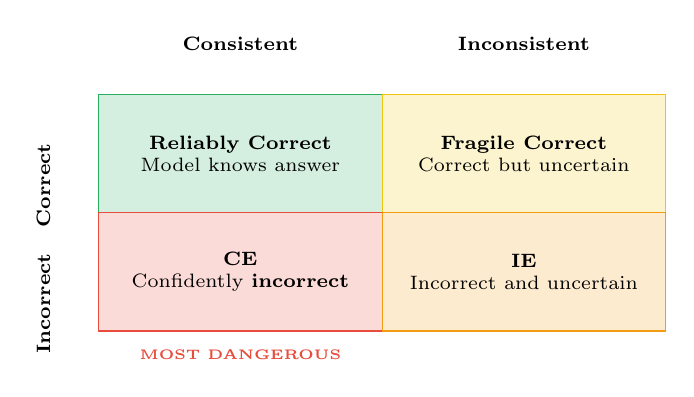
\begin{tikzpicture}[
    cell/.style={minimum width=3.6cm, minimum height=1.5cm, align=center, font=\scriptsize},
]
    \node[font=\scriptsize\bfseries] at (1.8, 2.6) {Consistent};
    \node[font=\scriptsize\bfseries] at (5.4, 2.6) {Inconsistent};
    \node[font=\scriptsize\bfseries, rotate=90] at (-0.7, 0.8) {Correct};
    \node[font=\scriptsize\bfseries, rotate=90] at (-0.7, -0.7) {Incorrect};
    \node[cell, fill=rcGreen!20, draw=rcGreen] at (1.8, 1.2)
        {\textbf{Reliably Correct}\\Model knows answer};
    \node[cell, fill=fcYellow!20, draw=fcYellow] at (5.4, 1.2)
        {\textbf{Fragile Correct}\\Correct but uncertain};
    \node[cell, fill=ceRed!20, draw=ceRed] at (1.8, -0.3)
        {\textbf{CE}\\Confidently \textbf{incorrect}};
    \node[cell, fill=ieOrange!20, draw=ieOrange] at (5.4, -0.3)
        {\textbf{IE}\\Incorrect and uncertain};
    \node[font=\tiny\bfseries, text=ceRed] at (1.8, -1.35) {MOST DANGEROUS};
\end{tikzpicture}
\caption{The $2\times 2$ error classification. Self-consistent errors
(CE) occupy the bottom-left cell: incorrect and showing no uncertainty.}
\label{fig:errormatrix}
\end{figure}

The pipeline architecture is shown in Figure~\ref{fig:pipeline}.

\begin{figure}[H]
\centering
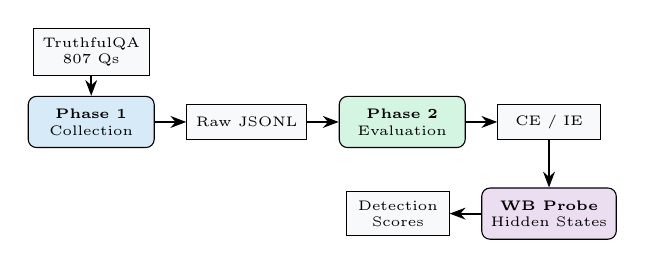
\begin{tikzpicture}[
    node distance=0.25cm and 0.4cm,
    box/.style={rectangle, draw, rounded corners=3pt, minimum width=1.6cm,
                minimum height=0.65cm, align=center, font=\tiny},
    data/.style={rectangle, draw, fill=lightbg, minimum width=1.3cm,
                 minimum height=0.45cm, align=center, font=\tiny},
    arrow/.style={-{Stealth[length=2mm]}, thick},
]
    \node[box, fill=phase1Blue!20] (p1) {\textbf{Phase~1}\\Collection};
    \node[data, right=of p1] (jsonl) {Raw JSONL};
    \node[box, fill=phase2Green!20, right=of jsonl] (p2) {\textbf{Phase~2}\\Evaluation};
    \node[data, right=of p2] (labels) {CE / IE};
    \node[box, fill=wbPurple!20, below=0.6cm of labels] (wb)
         {\textbf{WB Probe}\\Hidden States};
    \node[data, left=of wb] (scores) {Detection\\Scores};
    \node[data, above=0.25cm of p1] (tqa) {TruthfulQA\\807 Qs};
    \draw[arrow] (tqa) -- (p1);
    \draw[arrow] (p1) -- (jsonl);
    \draw[arrow] (jsonl) -- (p2);
    \draw[arrow] (p2) -- (labels);
    \draw[arrow] (labels) -- (wb);
    \draw[arrow] (wb) -- (scores);
\end{tikzpicture}
\caption{Two-phase pipeline. Phase~1 collects model outputs via APIs;
Phase~2 labels locally via NLI and judges. The white-box probe
operates on Phase~2 outputs.}
\label{fig:pipeline}
\end{figure}

\subsection{White-Box Cross-Model Probe (O2)}
\label{sec:method-wb}

The white-box probe addresses a practical constraint: every target
model in this study is accessed through an API that returns text
only. The hidden-state activations computed internally are not
exposed to the caller. Extracting the target model's own
representations is therefore infeasible for most models evaluated
here.

\textbf{Two Encoding Strategies.}
The study used two distinct strategies, depending on whether the
target model's weights are publicly accessible.

\textit{Original cross-model probing \citep{tan2025consistent}.}
This is the method as originally proposed: the target model is loaded
locally to extract its own hidden states directly. Every
question--answer pair is passed through the target, and the
last-token hidden state is extracted at each candidate layer.
Because these are the exact representations the model used to
generate the answer, they carry the most direct signal for error
detection. This approach was applied to Llama~4 Maverick~17B and
Qwen3 Next~80B, the two models whose weights are publicly available
and fit on the Nibi HPC cluster's A100 GPUs.

\textit{Extension: Proxy Encoding (this thesis's contribution).}
The baseline approach has two limitations. First, it cannot be
applied to closed-source API models (Claude Opus~4.6, GPT-5.2,
Grok~4, DeepSeek~V3.2), which do not expose hidden states. Second,
even when weights are available, many frontier models are too large
for typical research hardware.

To address both, this thesis proposes using a small local
open-weight model as a \emph{proxy encoder}. The proxy receives the
same question--answer text the target produced but shares no weights
or training with the target. If a small proxy can detect CEs
comparably to the target's own hidden states, then white-box-style
analysis becomes available for \emph{any} model regardless of
weight access or hardware constraints.
Two proxy encoder configurations were evaluated:
(a)~SmolLM3-3B (a compact 3B-parameter instruction-following model)
as response proxy, and (b)~Qwen3.5-4B (a 4B-parameter model from
Alibaba's Qwen series, providing a second architectural family) as
response proxy. In both cases, Phi-4-mini-instruct (a compact model
from Microsoft, architecturally distinct from both proxies) served
as the verifier. Full selection criteria are in
Appendix~\ref{app:wb-design}.

\textbf{Verifier Model.}
Regardless of encoding strategy, a second encoder called the
\emph{verifier} independently processes the same question--answer
pair. The verifier is always a different model from the response
encoder, so the two probes reflect complementary representations.
Different models encode factual knowledge differently; an error
undetectable in one model's hidden states may be detectable in
another's \citep{tan2025consistent}.

\textbf{Probe Architecture.}
For each question--answer pair, the last-token hidden state was
extracted from candidate layers of both the response encoder and the
verifier. A small feedforward neural network (FFN) probe (input
dimension $\to$ 256 $\to$ 128 $\to$ 64 $\to$ 1, with ReLU
activations and sigmoid output) was trained per layer using binary
cross-entropy loss, with CE as the positive class. The layer
achieving the highest validation AUROC was selected for each model.
This per-layer selection ensures that the most informative layer is
used regardless of network depth (Figure~\ref{fig:probe}).

\begin{figure}[H]
\centering
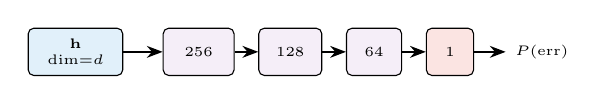
\begin{tikzpicture}[
    node distance=0.1cm,
    layer/.style={rectangle, draw, rounded corners=2pt,
                  minimum height=0.6cm, align=center, font=\tiny},
    arrow/.style={-{Stealth[length=2mm]}, thick},
]
    \node[layer, fill=phase1Blue!15, minimum width=1.2cm] (input)
         {$\mathbf{h}$\\dim=$d$};
    \node[layer, fill=wbPurple!10, minimum width=0.9cm, right=0.5cm of input]
         (l1) {256};
    \node[layer, fill=wbPurple!10, minimum width=0.8cm, right=0.3cm of l1]
         (l2) {128};
    \node[layer, fill=wbPurple!10, minimum width=0.7cm, right=0.3cm of l2]
         (l3) {64};
    \node[layer, fill=ceRed!15, minimum width=0.6cm, right=0.3cm of l3]
         (out) {1};
    \node[right=0.4cm of out, font=\tiny, align=center] (plabel) {$P(\text{err})$};
    \draw[arrow] (input) -- (l1);
    \draw[arrow] (l1) -- (l2);
    \draw[arrow] (l2) -- (l3);
    \draw[arrow] (l3) -- (out);
    \draw[arrow] (out) -- (plabel);
\end{tikzpicture}
\caption{FFN probe: $d \to 256 \to 128 \to 64 \to 1$. The best
layer per model is selected by validation AUROC. Output is
$P(\text{error})$.}
\label{fig:probe}
\end{figure}

\textbf{Cross-Model Score Fusion.}
Each question--answer pair receives two probe scores: $s_M$ from the
response encoder and $s_V$ from the verifier. These are combined as
$s = (1{-}\lambda)\,s_M + \lambda\,s_V$, where $\lambda \in [0,1]$
is selected by grid search on the validation set
(Figure~\ref{fig:fusion}). When $\lambda = 0$, the fused score
equals the response probe alone. Higher $\lambda$ indicates that the
verifier contributed meaningful complementary signal.

\begin{figure}[H]
\centering
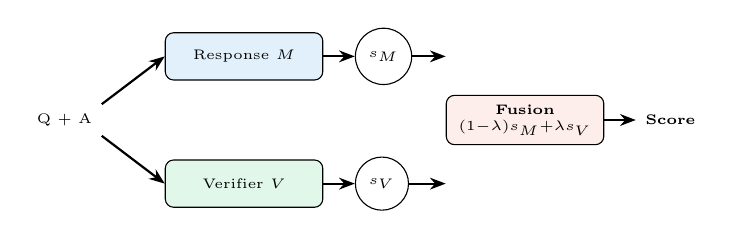
\begin{tikzpicture}[
    node distance=0.3cm and 0.5cm,
    box/.style={rectangle, draw, rounded corners=3pt,
                minimum width=2cm, minimum height=0.6cm,
                align=center, font=\tiny},
    score/.style={circle, draw, minimum size=0.5cm, font=\tiny},
    arrow/.style={-{Stealth[length=2mm]}, thick},
]
    \node[font=\tiny, align=center] (input) {Q + A};
    \node[box, fill=phase1Blue!15, above right=0.3cm and 0.8cm of input]
         (rm) {Response $M$};
    \node[score, right=0.4cm of rm] (sm) {$s_M$};
    \node[box, fill=phase2Green!15, below right=0.3cm and 0.8cm of input]
         (vm) {Verifier $V$};
    \node[score, right=0.4cm of vm] (sv) {$s_V$};
    \node[box, fill=ceRed!10, right=0.8cm of $(sm)!0.5!(sv)$]
         (fusion) {\textbf{Fusion}\\$(1{-}\lambda)s_M{+}\lambda s_V$};
    \node[right=0.4cm of fusion, font=\tiny\bfseries] (final) {Score};
    \draw[arrow] (input.north east) -- (rm.west);
    \draw[arrow] (input.south east) -- (vm.west);
    \draw[arrow] (rm) -- (sm);
    \draw[arrow] (vm) -- (sv);
    \draw[arrow] (sm.east) -- (fusion.west |- sm);
    \draw[arrow] (sv.east) -- (fusion.west |- sv);
    \draw[arrow] (fusion) -- (final);
\end{tikzpicture}
\caption{Cross-model fusion: two encoders, two probes, one combined
score. $\lambda = 0$ means the response encoder alone was optimal;
higher $\lambda$ means the verifier added signal.}
\label{fig:fusion}
\end{figure}

\textbf{Training Protocol.}
All probes used question-level train/validation/test splits of
80/10/10 with a fixed random seed. This prevents the same question from appearing in both training and
test, which would allow the probe to memorise question-specific
patterns rather than learning general error signals. Hidden states were Z-score normalised using training-set
statistics before being passed to the probe, ensuring features from
different layers and models are on a comparable scale. Each
configuration was run with three random seeds (11,~22,~33) to
estimate result stability. Training ran for up to 300 epochs with
early stopping on validation loss (patience~25), using the Adam
optimiser at a learning rate of $10^{-3}$. All experiments were
executed on the Nibi HPC cluster using NVIDIA A100 GPUs.

\subsection{Version-Evolution Study (O3)}
\label{sec:method-evo}

Three model families were selected for longitudinal analysis based on
the availability of at least four publicly accessible versions spanning
different release dates. The selection criteria were: (a) the family
must include models released across at least two calendar years,
(b) each version must be accessible via API or open weights, and
(c) the family must represent a distinct organization to ensure
diversity. The selected families, with four versions each, are:
\begin{itemize}[nosep]
\item \textbf{Grok} (xAI): Grok~3, Grok~4, Grok~4.1 Fast
      Reasoning, Grok~4.20 Beta 0309.
\item \textbf{Llama} (Meta): Llama~3~8B,
      3.1~8B, 3.3~70B, Llama~4 Maverick~17B.
\item \textbf{Qwen} (Alibaba): Qwen2.5~7B,
      2.5~72B, Qwen3~30B A3B, Qwen3 Next~80B.
\end{itemize}

Each model was evaluated on the same 807 TruthfulQA questions using
the same Phase~1 and Phase~2 protocol, yielding
$12 \times 807 = 9{,}684$ rows. For each question, the pipeline
produced one greedy answer and ten stochastic samples. CE was computed
with the same equivalence-only rule used throughout this thesis
($t{=}1.0$), so version-to-version comparisons are directly
comparable within each family.

The analysis focuses on CE trajectories across v1--v4 in each family,
using CE\% and CE/Wr as the primary indicators of whether newer
versions reduce self-consistent errors.

% ====================================================================
% 5. RESULTS
% ====================================================================
\section{Results}
\label{sec:results}

\subsection{Black-Box CE Rates (O1)}
\label{sec:results-bb}

Six frontier models were evaluated on 807 TruthfulQA questions each,
producing 4,842 rows. Per question: one greedy answer (temperature
$\approx 0.01$) and ten stochastic samples (temperature~$= 0.7$).
Correctness was determined by a three-judge ensemble; semantic
equivalence used hybrid NLI with GPT-5.2 fallback. All results
below use equivalence threshold $t{=}1.0$: all 10 stochastic
samples must match the greedy answer for a row to count as CE.

\subsubsection{Aggregate Results}

Table~\ref{tab:aggregate} summarizes the overall evaluation.
Of 4,842 rows, 63.3\% were correct, 32.2\% incorrect, and 4.5\% not
attempted. Among the 1,560 incorrect answers, 656 (42.1\%) were
self-consistent errors. This means that more than four in ten incorrect
answers were produced with full confidence and no variation across
all samples.

\begin{table}[H]
\centering
\footnotesize
\begin{tabular}{lrrr}
\toprule
 & Count & \% Total & \% Wrong \\
\midrule
Total rows    & 4,842 &        &       \\
Correct       & 3,063 & 63.3\% &       \\
Incorrect     & 1,560 & 32.2\% &       \\
Not attempted &   219 &  4.5\% &       \\
\midrule
CE            &   656 & 13.5\% & 42.1\% \\
IE            &   904 & 18.7\% & 57.9\% \\
\bottomrule
\end{tabular}
\caption{Aggregate results at $t{=}1.0$ across all six models.
CE = self-consistent error; IE = inconsistent error. 42.1\% of
incorrect answers are confident and repeatable.}
\label{tab:aggregate}
\end{table}

\subsubsection{Per-Model Breakdown}

Two metrics are used throughout this section. \textbf{CE\%} is the
CE rate: the number of CE rows divided by 807 (total questions per
model), expressing what fraction of all questions the model answered
with a confident wrong answer. \textbf{CE/Wr} is the CE-among-wrong
ratio: CE count divided by the number of incorrect answers, expressing
what fraction of the model's errors are self-consistent. A high
CE/Wr indicates that when the model is wrong, it tends to be
confidently and consistently wrong.

Table~\ref{tab:permodel} provides the full per-model breakdown. Models
are sorted by accuracy (descending). The Wrong, CE, and IE columns
show absolute counts out of 807 questions each.

\begin{table}[H]
\centering
\scriptsize
\setlength{\tabcolsep}{3pt}
\begin{tabular}{@{}lrrrrrr@{}}
\toprule
Model & Acc. & Wrong & CE & IE & CE\% & CE/Wr \\
\midrule
Claude Opus 4.6   & 74.7 & 169 &  91 &  78 & 11.3 & 53.8 \\
GPT-5.2           & 69.8 & 217 &  61 & 156 &  7.6 & 28.1 \\
Qwen3 Next 80B    & 65.2 & 247 & 148 &  99 & 18.3 & 59.9 \\
DeepSeek V3.2     & 60.3 & 276 & 143 & 133 & 17.7 & 51.8 \\
Grok 4            & 57.1 & 320 &  88 & 232 & 10.9 & 27.5 \\
Llama 4 Maverick  & 52.4 & 331 & 125 & 206 & 15.5 & 37.8 \\
\bottomrule
\end{tabular}
\caption{Per-model breakdown at $t{=}1.0$. Acc.\ = accuracy~(\%);
Wrong = incorrect count; CE/IE = error type counts; CE\% = CE rate
(CE/807); CE/Wr = CE as~\% of incorrect answers.}
\label{tab:permodel}
\end{table}

Figure~\ref{fig:cebar} visualizes the CE rate alongside the
CE-among-wrong ratio for each model.

\begin{figure}[H]
\centering
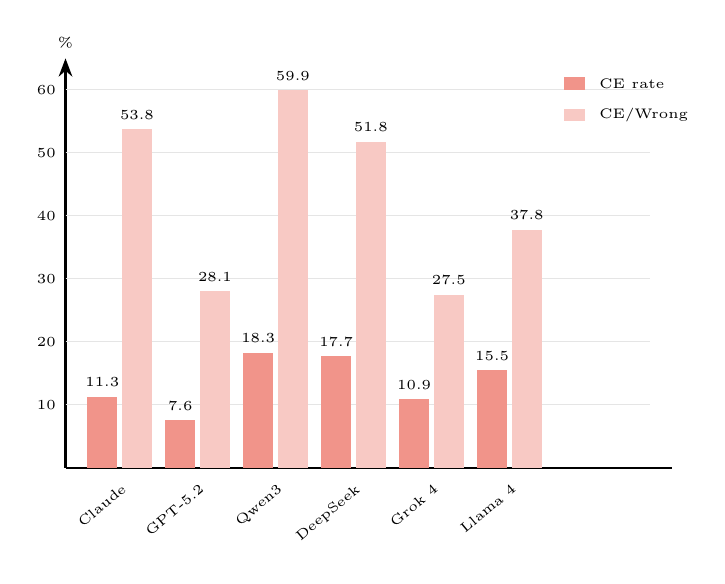
\begin{tikzpicture}[yscale=0.08, xscale=0.55]
    \draw[thick, -{Stealth}] (0,0) -- (0, 65)
         node[above, font=\tiny] {\%};
    \draw[thick] (0,0) -- (14,0);
    \foreach \y in {10,20,30,40,50,60} {
        \draw[gray!20] (0,\y) -- (13.5,\y);
        \node[left, font=\tiny] at (0,\y) {\y};
    }
    % CE rate bars (red)
    \fill[ceRed!60] (0.5,0) rectangle (1.2, 11.3);
    \fill[ceRed!60] (2.3,0) rectangle (3.0, 7.6);
    \fill[ceRed!60] (4.1,0) rectangle (4.8, 18.3);
    \fill[ceRed!60] (5.9,0) rectangle (6.6, 17.7);
    \fill[ceRed!60] (7.7,0) rectangle (8.4, 10.9);
    \fill[ceRed!60] (9.5,0) rectangle (10.2, 15.5);
    % CE/Wrong bars (darker, offset)
    \fill[ceRed!30] (1.3,0) rectangle (2.0, 53.8);
    \fill[ceRed!30] (3.1,0) rectangle (3.8, 28.1);
    \fill[ceRed!30] (4.9,0) rectangle (5.6, 59.9);
    \fill[ceRed!30] (6.7,0) rectangle (7.4, 51.8);
    \fill[ceRed!30] (8.5,0) rectangle (9.2, 27.5);
    \fill[ceRed!30] (10.3,0) rectangle (11.0, 37.8);
    % Labels
    \node[below, font=\tiny, rotate=40, anchor=north east] at (1.3,-0.3) {Claude};
    \node[below, font=\tiny, rotate=40, anchor=north east] at (3.1,-0.3) {GPT-5.2};
    \node[below, font=\tiny, rotate=40, anchor=north east] at (4.9,-0.3) {Qwen3};
    \node[below, font=\tiny, rotate=40, anchor=north east] at (6.7,-0.3) {DeepSeek};
    \node[below, font=\tiny, rotate=40, anchor=north east] at (8.5,-0.3) {Grok 4};
    \node[below, font=\tiny, rotate=40, anchor=north east] at (10.3,-0.3) {Llama 4};
    % Value labels for CE rate
    \node[above, font=\tiny] at (0.85, 11.3) {11.3};
    \node[above, font=\tiny] at (2.65, 7.6) {7.6};
    \node[above, font=\tiny] at (4.45, 18.3) {18.3};
    \node[above, font=\tiny] at (6.25, 17.7) {17.7};
    \node[above, font=\tiny] at (8.05, 10.9) {10.9};
    \node[above, font=\tiny] at (9.85, 15.5) {15.5};
    % Value labels for CE/Wrong
    \node[above, font=\tiny] at (1.65, 53.8) {53.8};
    \node[above, font=\tiny] at (3.45, 28.1) {28.1};
    \node[above, font=\tiny] at (5.25, 59.9) {59.9};
    \node[above, font=\tiny] at (7.05, 51.8) {51.8};
    \node[above, font=\tiny] at (8.85, 27.5) {27.5};
    \node[above, font=\tiny] at (10.65, 37.8) {37.8};
    % Legend
    \fill[ceRed!60] (11.5, 60) rectangle (12.0, 62);
    \node[right, font=\tiny] at (12.1, 61) {CE rate};
    \fill[ceRed!30] (11.5, 55) rectangle (12.0, 57);
    \node[right, font=\tiny] at (12.1, 56) {CE/Wrong};
\end{tikzpicture}
\caption{CE rate~(\%, dark bars) and CE-among-wrong ratio~(\%, light
bars) by model at $t{=}1.0$. Higher accuracy does not guarantee lower
CE: Qwen3 has the highest CE-among-wrong (59.9\%) despite mid-range
accuracy.}
\label{fig:cebar}
\end{figure}

\subsubsection{Key Observations}

\begin{itemize}[nosep]
\item \textbf{CEs are common across all models.} CE rates range from
      7.6\% (GPT-5.2) to 18.3\% (Qwen3 Next~80B). No model is
      CE-free.
\item \textbf{Accuracy does not predict CE rate.} Claude has the
      highest accuracy (74.7\%) but the third-highest CE rate
      (11.3\%). GPT-5.2 has the lowest CE rate (7.6\%) at lower
      accuracy (69.8\%) than Claude.
\item \textbf{Models differ in error rigidity.}
      The CE-among-wrong ratio ranges from 27.5\% (Grok~4) to 59.9\%
      (Qwen3 Next~80B). Claude and Qwen exhibit the highest ratios
      (53.8\% and 59.9\%), indicating that when these models produce
      an incorrect answer, it is predominantly a single repeated
      response. GPT-5.2 and Grok~4 have substantially lower ratios
      ($\sim$28\%), indicating that their errors tend to vary across
      samples.
\item \textbf{Error volume varies substantially.} Incorrect-answer counts
      range from 169 (Claude) to 331 (Llama~4). Llama and Grok
      produce the highest total error counts but a smaller fraction of
      these errors are self-consistent, whereas Claude and Qwen produce
      fewer errors overall but a larger proportion of them are
      consistently incorrect.
\item \textbf{CE and IE are complementary error modes.} Across the six
      models, CE accounts for 42.1\% of all errors and IE for 57.9\%
      (Table~\ref{tab:aggregate}). These two error types partition the
      full set of incorrect answers: CE represents the confident
      failure mode, and IE represents the uncertain failure mode.
\end{itemize}

\subsection{Cross-Model Overlap and Category Analysis}
\label{sec:results-overlap}

\subsubsection{Pairwise CE Overlap}

The per-model results show that CE is common across all six models,
but they do not tell us whether different models are making the
\emph{same} mistakes. If two models consistently fail on the same
questions with the same wrong answer, this points to shared
misconceptions absorbed from common training data. If, on the other
hand, CE errors are largely model-specific, then cross-model
comparison becomes a viable detection strategy, an idea explored
by \citet{tan2025consistent}. To investigate this, pairwise CE
overlap was computed for all 15 model pairs at $t{=}1.0$.
For each pair, Table~\ref{tab:ce_overlap} lists CE counts, the
number of shared CE questions (\emph{Both}), Jaccard similarity,
and the fraction of shared-CE questions where both models gave the
same incorrect greedy answer (SW\%, determined via NLI hybrid
equivalence).

\begin{table}[H]
\centering
\resizebox{\columnwidth}{!}{%
\begin{tabular}{@{}llrrrrrr@{}}
\toprule
Model A & Model B & $A_{\mathrm{CE}}$ & $B_{\mathrm{CE}}$ & Both &
Jacc. & Same & SW\% \\
\midrule
DeepSeek    & Qwen3 Next  & 143 & 148 & 77 & .360 & 59 & 76.6 \\
DeepSeek    & Llama 4     & 143 & 125 & 71 & .360 & 53 & 74.6 \\
Llama 4     & Qwen3 Next  & 125 & 148 & 69 & .338 & 56 & 81.2 \\
Claude      & DeepSeek    &  91 & 143 & 60 & .345 & 41 & 68.3 \\
DeepSeek    & Grok 4      & 143 &  88 & 51 & .283 & 33 & 64.7 \\
Grok 4      & Qwen3 Next  &  88 & 148 & 50 & .269 & 39 & 78.0 \\
Grok 4      & Llama 4     &  88 & 125 & 45 & .268 & 32 & 71.1 \\
Claude      & Llama 4     &  91 & 125 & 43 & .249 & 28 & 65.1 \\
Claude      & Qwen3 Next  &  91 & 148 & 43 & .219 & 30 & 69.8 \\
GPT-5.2     & Qwen3 Next  &  61 & 148 & 39 & .229 & 31 & 79.5 \\
Claude      & Grok 4      &  91 &  88 & 38 & .270 & 25 & 65.8 \\
DeepSeek    & GPT-5.2     & 143 &  61 & 38 & .229 & 28 & 73.7 \\
GPT-5.2     & Llama 4     &  61 & 125 & 36 & .240 & 26 & 72.2 \\
Claude      & GPT-5.2     &  91 &  61 & 30 & .246 & 22 & 73.3 \\
GPT-5.2     & Grok 4      &  61 &  88 & 30 & .252 & 26 & 86.7 \\
\midrule
\multicolumn{4}{@{}l}{\textbf{Sum / overall}} &
\textbf{720} & \textbf{.277} & \textbf{529} & \textbf{73.5} \\
\bottomrule
\end{tabular}}
\caption{Pairwise CE overlap at $t{=}1.0$ (NLI hybrid). Same: same
greedy wrong answer; SW\%: Same/Both$\times$100. Totals: 720 shared
CE instances, 529 same-wrong (73.5\%).}
\label{tab:ce_overlap}
\end{table}

Three observations follow.
\begin{itemize}[nosep]
\item \textbf{CE overlap is limited.} Pairwise Jaccard ranges from
      0.219 to 0.360 (mean 0.277), meaning 64--78\% of each pair's CE
      union is not shared. This is consistent with
      \citet{tan2025consistent}, who reported limited pairwise CE
      overlap (up to ${\sim}$29\%) on TriviaQA and SciQ. Most CE
      failures are model-specific, which supports the viability of
      cross-model detection methods.
\item \textbf{Open-weight models overlap more.} The three
      open-weight models (DeepSeek, Llama~4, Qwen3 Next) have the
      highest pairwise Jaccard scores (0.34--0.36), while
      closed--open pairs are typically lower (${\sim}$0.22--0.28).
      This suggests that shared training corpora or architectural
      similarities drive error alignment.
\item \textbf{Shared CEs usually involve the same wrong answer.} Of
      the 720 shared-CE instances across all pairs, 529 (73.5\%)
      involve the same incorrect greedy answer. When two models do
      fail on the same question, they tend to converge on the same
      misconception rather than producing different wrong answers.
      The union of CE questions across all six models covers 292
      distinct items (36.2\% of 807), confirming that the
      ``dangerous question'' set is broad and model-dependent.
\end{itemize}

\subsubsection{Category-Level CE Vulnerability}

Each of the 807 TruthfulQA questions belongs to one of 38 topical
categories defined in the original dataset
\citep{lin2022truthfulqa}. To identify which domains are most
vulnerable to self-consistent errors, the 4,842 evaluated rows were
joined with TruthfulQA category labels (4,842 of 4,842 matched) and
CE rates were computed per category across all six models.
Table~\ref{tab:ce_category} reports the ten highest and five lowest
CE-rate categories (restricted to categories with $\geq 30$ rows
for statistical stability).

\begin{table}[H]
\centering
\scriptsize
\setlength{\tabcolsep}{3pt}
\begin{tabular}{@{}lrrrrr@{}}
\toprule
Category & Rows & CE & IE & CE\% & CE/Wr\% \\
\midrule
\multicolumn{6}{@{}l}{\textit{Top 10 by CE rate}} \\
Confusion: People     & 138 & 69 &  20 & 50.0 & 77.5 \\
Confusion: Other      &  48 & 22 &   7 & 45.8 & 75.9 \\
Misquotations         &  90 & 35 &   7 & 38.9 & 83.3 \\
Advertising           &  78 & 26 &  20 & 33.3 & 56.5 \\
Education             &  60 & 19 &  12 & 31.7 & 61.3 \\
Distraction           &  84 & 25 &  30 & 29.8 & 45.5 \\
Proverbs              & 102 & 29 &  16 & 28.4 & 64.4 \\
Psychology            & 108 & 28 &  36 & 25.9 & 43.8 \\
Science               &  54 & 10 &  16 & 18.5 & 38.5 \\
Indexical Err: Loc.   &  66 & 12 &   9 & 18.2 & 57.1 \\
\midrule
\multicolumn{6}{@{}l}{\textit{Bottom 5 by CE rate}} \\
Logical Falsehood     &  78 &  2 &   6 &  2.6 & 25.0 \\
Mandela Effect        &  36 &  1 &   1 &  2.8 & 50.0 \\
Conspiracies          & 150 &  1 &  13 &  0.7 &  7.1 \\
Politics              &  60 &  0 &   2 &  0.0 &  0.0 \\
Statistics            &  30 &  0 &   1 &  0.0 &  0.0 \\
\bottomrule
\end{tabular}
\caption{CE rates by TruthfulQA category at $t{=}1.0$ (all six
models combined). Rows: total (question, model) pairs; CE\%: CE
rate; CE/Wr\%: CE as fraction of all incorrect answers. Categories
with $\geq 30$ rows shown.}
\label{tab:ce_category}
\end{table}

The category analysis reveals that CE vulnerability varies
dramatically by topic. Three observations follow.

\begin{itemize}[nosep]
\item \textbf{Confusion and misquotation categories are most
      CE-prone.} ``Confusion: People'' has a CE rate of 50.0\%,
      meaning half of all responses in this category are confident
      and incorrect. These questions typically ask about commonly
      confused individuals (e.g., which president signed a particular
      law), where models have memorised an incorrect association and
      reproduce it consistently. ``Misquotations'' shows a CE rate of
      38.9\% with the highest CE-among-wrong ratio (83.3\%): when the
      model produces an incorrect quote attribution, it nearly always
      repeats the same incorrect attribution.
\item \textbf{Conspiracies, politics, and statistics are nearly
      CE-free.} Conspiracies has a CE rate of only 0.7\% (1 of 150),
      and Politics and Statistics have zero CEs. These categories
      involve questions where models have likely been trained to
      hedge, refuse, or express uncertainty, producing inconsistent
      rather than self-consistent errors.
\item \textbf{High CE/Wr\% indicates error rigidity.} Categories
      such as Misquotations (83.3\%), Confusion: People (77.5\%), and
      Proverbs (64.4\%) show that when models produce incorrect answers in these
      domains, the error is overwhelmingly self-consistent. This
      signals that these are memorised misconceptions rather than
      noisy guesses.
\end{itemize}

\subsection{White-Box Probe Results (O2)}
\label{sec:results-wb}

White-box experiments comprised 17 probe runs on the Nibi HPC
cluster, organised into two groups: (a)~two proxy configurations
covering all six target models (this thesis's contribution), and
(b)~five original cross-model probing runs for the two open-weight
models (replicating \citealp{tan2025consistent}).

\subsubsection{Proxy Configuration~1: SmolLM3-3B + Phi-4-mini}

Table~\ref{tab:wb_smollm} presents CE metrics for SmolLM3-3B as
response proxy with Phi-4-mini-instruct as verifier. The probe
achieves strong CE detection (AUROC 0.85--1.00, mean~0.93) despite
using proxy encoders rather than the target models' own hidden
states. The $\lambda$ column shows the fusion weight assigned to the
verifier: $\lambda = 0$ means the target-only probe was already
optimal; higher values indicate the verifier added signal.

\begin{table}[H]
\centering
\scriptsize
\begin{tabular}{lrrrrl}
\toprule
Target & Tgt & Ver & Fused & $\lambda$ & Test \\
\midrule
Claude 4.6  & .952 & \textbf{1.00} & .985 & .27 & 15C/6CE \\
DeepSeek    & .852 & \textbf{.878} & .875 & .97 & 8C/16CE \\
GPT-5.2     & .935 & \textbf{.972} & .935 & .00 & 6C/6CE \\
Grok 4      & .923 & \textbf{.949} & .923 & .00 & 3C/13CE \\
Llama 4     & \textbf{.877} & .858 & \textbf{.877} & .00 & 9C/13CE \\
Qwen3 Next  & \textbf{.915} & .884 & .914 & .45 & 16C/14CE \\
\midrule
\textbf{Mean} & .909 & .923 & .918 & & \\
\bottomrule
\end{tabular}
\caption{CE AUROC for SmolLM3-3B + Phi-4-mini across all six targets.
Tgt = target-only AUROC; Ver = verifier-only AUROC; Fused = fusion
score; $\lambda$ = verifier weight in fusion; Test = number of
correct (C) and CE items in the held-out test partition (e.g.\
15C/6CE means 15 correct rows and 6 CE rows). Bold marks the best
variant per target.}
\label{tab:wb_smollm}
\end{table}

\subsubsection{Proxy Configuration~2: Qwen3.5-4B + Phi-4-mini}

Table~\ref{tab:wb_qwen} shows a second proxy configuration using
Qwen3.5-4B. Performance is comparable: the verifier achieves
perfect CE AUROC (1.00) on Claude, and fusion with
$\lambda = 0.5$ also reaches 1.00 for Claude.

\begin{table}[H]
\centering
\scriptsize
\begin{tabular}{lrrrrl}
\toprule
Target & Tgt & Ver & Fused & $\lambda$ & Test \\
\midrule
Claude 4.6  & .941 & \textbf{1.00} & \textbf{1.00} & .50 & 15C/6CE \\
DeepSeek    & .844 & \textbf{.878} & .846 & .05 & 8C/16CE \\
GPT-5.2     & .954 & \textbf{.972} & .954 & .00 & 6C/6CE \\
Grok 4      & .897 & \textbf{.949} & .897 & .00 & 3C/13CE \\
Llama 4     & \textbf{.880} & .858 & .877 & .03 & 9C/13CE \\
Qwen3 Next  & \textbf{.942} & .884 & .940 & .25 & 16C/14CE \\
\midrule
\textbf{Mean} & .910 & .923 & .919 & & \\
\bottomrule
\end{tabular}
\caption{CE AUROC for Qwen3.5-4B + Phi-4-mini. Column definitions
as in Table~\ref{tab:wb_smollm}. Both proxy configurations yield
comparable mean performance ($\sim$0.92).}
\label{tab:wb_qwen}
\end{table}

\subsubsection{Original Cross-Model Probing \citep{tan2025consistent}}

For the two open-weight models (Llama~4 Maverick~17B and Qwen3
Next~80B), the original method of \citet{tan2025consistent} was
applied: each target model was loaded locally and its own hidden
states were extracted directly. These runs serve as the baseline
against which the proxy approach is compared.
Table~\ref{tab:wb_baseline} reports all five configurations.

\begin{table}[H]
\centering
\scriptsize
\begin{tabular}{llrrrr}
\toprule
Target & Verifier & Tgt & Ver & Fused & $\lambda$ \\
\midrule
Llama 4 & Llama-3.1-8B     & .872 & \textbf{.895} & .872 & .08 \\
Llama 4 & Qwen2.5-0.5B     & \textbf{.872} & .866 & \textbf{.872} & .00 \\
Llama 4 & Qwen3-Next-80B   & .872 & \textbf{.909} & .883 & .18 \\
\midrule
Qwen3 Next & Llama-3.1-8B  & \textbf{.946} & .929 & .936 & .92 \\
Qwen3 Next & Qwen2.5-0.5B  & \textbf{.946} & .924 & \textbf{.946} & .53 \\
\bottomrule
\end{tabular}
\caption{Original cross-model probing \citep{tan2025consistent}: target
model encodes its own answers. Tgt = target-only AUROC; Ver =
verifier-only; Fused = cross-model fusion.}
\label{tab:wb_baseline}
\end{table}

Target-only performance is stable within each target (.872 for
Llama~4; .946 for Qwen3 Next). For Llama~4, the Qwen3-Next
verifier is strongest (Ver=.909), and fusion improves CE AUROC from
.872 to .883. For Qwen3 Next, both verifiers score below
target-only, and fusion does not exceed .946.

Comparing these baselines (target-only AUROC 0.87--0.95) with the
proxy results (0.84--0.95) validates the proxy approach: the
difference is at most 0.03 AUROC. A 3B--4B proxy encoder can
substitute for the target's own hidden states with minimal loss,
making CE detection feasible for closed-source APIs and for
open-weight models too large to run locally.

\subsubsection{Key Observations}

\begin{itemize}[nosep]
\item \textbf{The verifier dominates CE detection for most targets.}
      The verifier-only probe achieved the highest CE AUROC for four
      of six targets (Claude, DeepSeek, GPT-5.2, Grok) in both proxy
      configurations, confirming that a second model's representation
      encodes error signals absent from the response model's own
      hidden states.
\item \textbf{Fusion helps selectively.} The fused score matched or
      improved the best single-model probe for DeepSeek
      ($\lambda = 0.97$) and Claude ($\lambda = 0.50$, reaching
      perfect AUROC). For other targets, $\lambda = 0$ indicates the
      target-only probe was already optimal.
\item \textbf{Proxy encoders match the baseline.} Comparing proxy
      runs against the original cross-model probing runs shows at most 0.03
      AUROC difference. Small proxy encoders (3B--4B) can substitute
      for the target's own hidden states, enabling CE detection for
      closed-source APIs and large open-weight models.
\item \textbf{Small test partitions warrant caution.} Several CE
      test sets contain few samples (GPT-5.2: 12~items; Grok~4:
      16~items), so near-perfect AUROC values carry high variance.
      Larger-scale replication is needed to establish tighter
      confidence intervals.
\end{itemize}

\subsection{Version-Evolution Results (O3)}
\label{sec:results-evo}

Table~\ref{tab:evolution} presents the version-evolution results at
$t{=}1.0$. The 12~models span April~2024 to March~2026, covering
two years of development across three families (9,684~rows total).
The CE/Wr column shows what fraction of each model's incorrect
answers are self-consistent.

\begin{table}[H]
\centering
\tiny
\setlength{\tabcolsep}{2.5pt}
\begin{tabular}{@{}llcrrrrc@{}}
\toprule
 & Model & Date & Acc. & CE & IE & CE\% & CE/Wr \\
\midrule
\multicolumn{8}{@{}l}{\textit{Grok (xAI): closed, large-scale}} \\
v1 & Grok 3            & 2025-06 & 56.8 & 143 & 175 & 17.7 & 45.0 \\
v2 & Grok 4            & 2025-07 & 57.1 &  88 & 232 & 10.9 & 27.5 \\
v3 & Grok 4.1 Fast R.  & 2025-11 & 71.3 &  48 & 153 &  5.9 & 23.9 \\
v4 & Grok 4.20 Beta    & 2026-03 & 79.7 &   4 & 133 &  0.5 &  2.9 \\
\midrule
\multicolumn{8}{@{}l}{\textit{Llama (Meta): open-weight, mixed scale}} \\
v1 & Llama 3 8B        & 2024-04 & 38.7 &  79 & 368 &  9.8 & 17.7 \\
v2 & Llama 3.1 8B      & 2024-07 & 43.7 &  58 & 331 &  7.2 & 14.9 \\
v3 & Llama 3.3 70B     & 2024-12 & 52.3 & 141 & 191 & 17.5 & 42.5 \\
v4 & Llama 4 Mav.\ 17B & 2025-04 & 52.4 & 125 & 206 & 15.5 & 37.8 \\
\midrule
\multicolumn{8}{@{}l}{\textit{Qwen (Alibaba): open-weight, mixed scale}} \\
v1 & Qwen2.5 7B        & 2024-09 & 45.8 & 107 & 285 & 13.3 & 27.3 \\
v2 & Qwen2.5 72B       & 2024-11 & 57.4 & 139 & 162 & 17.2 & 46.2 \\
v3 & Qwen3 30B A3B     & 2025-07 & 58.1 & 101 & 197 & 12.5 & 33.9 \\
v4 & Qwen3 Next 80B    & 2025-09 & 65.2 & 148 &  99 & 18.3 & 59.9 \\
\bottomrule
\end{tabular}
\caption{Version-evolution at $t{=}1.0$. Acc.\ = accuracy~(\%);
CE/IE = error counts; CE\% = CE rate; CE/Wr = CE as~\% of incorrect
answers. Grok shows monotonic CE decline; Llama and Qwen do not.}
\label{tab:evolution}
\end{table}

\textbf{Trends.}
The three families show distinctly different CE trajectories:
\begin{itemize}[nosep]
\item \textbf{Grok:} $17.7\% \to 10.9\% \to 5.9\% \to 0.5\%$.
      Monotonic improvement at every step. Accuracy also rose from
      56.8\% to 79.7\%. Grok~4.20 Beta (March~2026) is nearly
      CE-free: the CE-among-wrong ratio dropped from 45.0\% to 2.9\%,
      meaning almost none of its remaining errors are self-consistent.
      Cumulative CE reduction from v1 to v4 is 17.2~pp
      ($p \approx 0$).
\item \textbf{Llama:} $9.8\% \to 7.2\% \to 17.5\% \to 15.5\%$.
      Non-monotonic. The v1$\to$v2 step improved CE, but v2$\to$v3
      (8B to 70B) produced a sharp 10.3~pp increase. The
      CE-among-wrong ratio rose from 14.9\% to 42.5\% at this scale
      transition, indicating the larger model became more confident in
      its errors. The v3$\to$v4 step (70B to 17B MoE) showed a
      slight recovery that was not statistically significant
      ($p = 0.40$).
\item \textbf{Qwen:} $13.3\% \to 17.2\% \to 12.5\% \to 18.3\%$.
      Non-monotonic, alternating direction at each step. The
      CE-among-wrong ratio rose from 27.3\% (7B) to 59.9\% (80B):
      the largest model produces fewer errors overall, but a greater
      proportion of them are self-consistent.
\end{itemize}

Across all three families, accuracy improved consistently (every
v4 is more accurate than its v1), yet CE reduction did not follow
automatically. This confirms that accuracy and CE are partially
orthogonal metrics.

Figure~\ref{fig:timeline} visualizes these trajectories.

\begin{figure}[H]
\centering
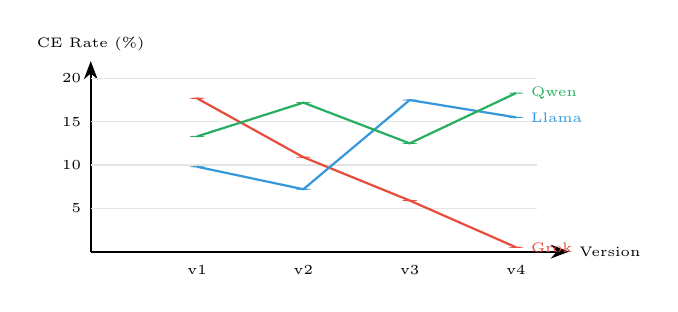
\begin{tikzpicture}[xscale=1.35, yscale=0.11]
    \draw[thick, -{Stealth}] (0,0) -- (0, 22)
         node[above, font=\tiny] {CE Rate (\%)};
    \draw[thick, -{Stealth}] (0,0) -- (4.5, 0)
         node[right, font=\tiny] {Version};
    \foreach \y in {5,10,15,20} {
        \draw[gray!20] (0,\y) -- (4.2,\y);
        \node[left, font=\tiny] at (0,\y) {\y};
    }
    \foreach \x/\l in {1/v1,2/v2,3/v3,4/v4} {
        \node[below, font=\tiny] at (\x, -0.5) {\l};
    }
    \draw[thick, ceRed] plot coordinates {(1,17.7)(2,10.9)(3,5.9)(4,0.5)};
    \node[right, font=\tiny, text=ceRed] at (4.05, 0.5) {Grok};
    \draw[thick, phase1Blue] plot coordinates {(1,9.8)(2,7.2)(3,17.5)(4,15.5)};
    \node[right, font=\tiny, text=phase1Blue] at (4.05, 15.5) {Llama};
    \draw[thick, rcGreen] plot coordinates {(1,13.3)(2,17.2)(3,12.5)(4,18.3)};
    \node[right, font=\tiny, text=rcGreen] at (4.05, 18.3) {Qwen};
    \foreach \x/\y in {1/17.7,2/10.9,3/5.9,4/0.5}
        \fill[ceRed] (\x,\y) circle (2pt);
    \foreach \x/\y in {1/9.8,2/7.2,3/17.5,4/15.5}
        \fill[phase1Blue] (\x,\y) circle (2pt);
    \foreach \x/\y in {1/13.3,2/17.2,3/12.5,4/18.3}
        \fill[rcGreen] (\x,\y) circle (2pt);
\end{tikzpicture}
\caption{CE rate (\%) over model versions at $t{=}1.0$. Grok shows
clear monotonic decline; Llama and Qwen oscillate.}
\label{fig:timeline}
\end{figure}

All results in this section use equivalence threshold
($t{=}1.0$): every stochastic sample must match the greedy answer for
a row to count as CE. Sensitivity analysis at lower thresholds
($t \in \{0.7, 0.8, 0.9\}$) is provided in
Appendix~\ref{app:thresholds}; the trend patterns are unchanged.

\textbf{Key Takeaway.}
Grok is the only family with clear CE reduction across generations.
Its version trajectory is also the cleanest to interpret: all four
versions are large closed models from a single laboratory with no
disclosed parameter-count changes, so CE changes cannot be attributed
to scale. For Llama and Qwen, CE changes are \emph{confounded}
(i.e.\ mixed with other factors) by parameter-scale differences
(8B$\to$70B for Llama; 7B$\to$72B$\to$30B$\to$80B for Qwen),
making it difficult to separate generational training improvement
from the effect of simply using a larger model.

\subsection{Novelty of Results}
\label{sec:results-novelty}

Taken together, these results extend prior work in three ways: they
measure CE in closed-source frontier models for the first time,
demonstrate that proxy-based probing makes cross-model detection
feasible without weight access, and provide the first longitudinal
view of CE evolution across model generations. How these findings
relate to the existing literature, and their practical implications,
are discussed in Section~\ref{sec:discussion}.

% ====================================================================
% 6. DISCUSSION
% ====================================================================
\section{Discussion}
\label{sec:discussion}

\subsection{Threats to Validity}
\label{sec:discussion-threats}

\textbf{Small white-box test sets.} A few CE test partitions are
very small (e.g., GPT-5.2 has only 12 test items). High AUROC on
a small test set is not very reliable, so the white-box results
should be interpreted cautiously and replicated at larger scale.

\textbf{Single benchmark.} Everything here is on TruthfulQA. The
results may not carry over to other tasks or datasets.

\subsection{Implications for Research}
\label{sec:discussion-research}

The main takeaway from the black-box results is that 42\% of
incorrect answers are self-consistent, and accuracy alone does not
predict this. DeepSeek~V3.2 (60.3\% accuracy) and Grok~4 (57.1\%
accuracy) are only 3.2~pp apart in accuracy but 6.8~pp apart in CE
rate. This supports \citet{tan2025consistent}'s argument that CE
should be tracked as a separate metric alongside accuracy.

The proxy probing results show that white-box detection is not
limited to open-weight models. A 3B-parameter local model can
produce hidden-state features that are informative enough to detect
CEs in much larger closed-source targets. This suggests that the
signal for a factual error lives in the text itself and is not
specific to any one model's internal representations.

The version-evolution results extend what \citet{tan2025consistent}
found about scale: not only do CEs not decrease when a model gets
larger, they also do not reliably decrease across generations, even
when accuracy goes up. Grok is the exception, and it suggests
that CE reduction is possible if it is explicitly targeted during
training, perhaps through reasoning-based methods.

\subsection{Implications for Practice}
\label{sec:discussion-practice}

Systems that check model consistency by sampling multiple answers
will miss CEs entirely, because a CE produces the same wrong answer
every time \citep{tan2025consistent, manakul2023selfcheckgpt}. This
matters most in high-stakes settings like healthcare, legal advice,
or education, where repeated agreement can give a user false
confidence in an incorrect answer.

Grok~4.20's near-zero CE rate (0.5\%) shows that it is possible to
get CE down to very low levels. Other developers can use this as a
benchmark to aim for. For anyone deploying an API-based model,
proxy-based probing offers a practical monitoring approach: run a
small local encoder on a sample of production queries periodically
to estimate whether CE rates are changing, without needing access
to the model's internals.

\subsection{Limitations}
\label{sec:discussion-limits}

Two limitations beyond those already noted: the three-judge ensemble
reduces individual bias but the three providers may still share some
systematic blind spots. The proxy probing results are also a
lower bound; if the target model's own hidden states were accessible,
detection would likely be somewhat better.

\textbf{Ethics.} TruthfulQA includes questions about health, law,
and conspiracies. A model that confidently repeats a wrong medical
fact across every response is a real safety concern. No
personally identifiable data was used in this study; all questions
are from a publicly available benchmark.

\subsection{Generalisability}
\label{sec:discussion-general}

The pipeline itself (two-phase collection, hybrid NLI equivalence
checking, CE/IE labelling) is not specific to TruthfulQA. It should
work on any closed-book QA benchmark that provides reference answers,
such as TriviaQA or SciQ \citep{tan2025consistent}. The
proxy-based probing approach applies to any model accessible via
API. The version-evolution protocol applies to any family with at
least a few publicly accessible versions.

That said, TruthfulQA is specifically designed to elicit
misconceptions, so CE rates here are probably higher than on a
general-purpose benchmark. All six black-box models are
frontier-scale, so results may not extend to smaller or
specialised models. The proxy probing has only been tested on
short factual answers; using it for long-form generation would
require a different hidden-state extraction strategy, such as
pooling across all output tokens rather than taking just the last
one \citep{lin2022truthfulqa}.

% ====================================================================
% 7. CONCLUSIONS
% ====================================================================
\section{Conclusions}
\label{sec:conclusions}

LLMs regularly produce hallucinations \citep{ji2023hallucination},
and a particularly dangerous subtype, self-consistent errors (CEs),
remains undetectable by output-based consistency methods
\citep{tan2025consistent}. This thesis addressed three objectives:
measuring CE prevalence (O1), detecting CEs via cross-model probes
(O2), and tracking CE evolution over model generations (O3).

\textbf{CE is common.} 42.1\% of incorrect answers were
self-consistent at $t{=}1.0$ (Table~\ref{tab:aggregate}), with
per-model CE rates from 7.6\% to 18.3\%
(Table~\ref{tab:permodel}). Higher accuracy does not guarantee
fewer CEs.

\textbf{White-box probes detect CEs effectively.} Proxy-based
cross-model probes achieved CE AUROC of 0.85--1.00 across all six
targets (Tables~\ref{tab:wb_smollm}--\ref{tab:wb_qwen}). The
verifier probe was strongest for four of six targets, confirming
that different models encode complementary error signals.

\textbf{CE evolution is not automatic.} Only Grok showed monotonic
CE reduction (17.7\%~$\to$~0.5\%). Llama and Qwen showed
non-monotonic patterns (Table~\ref{tab:evolution},
Figure~\ref{fig:timeline}).

These findings address O1--O3 and support the conclusion that
self-consistent errors require explicit measurement and monitoring
in model development, alongside standard accuracy reporting.

% ====================================================================
% 8. FUTURE WORK AND LESSONS LEARNT
% ====================================================================
\section{Future Work and Lessons Learnt}
\label{sec:future}

\subsection{Future Work}

\textbf{Multi-benchmark extension.} Replicating the pipeline on
TriviaQA, SciQ, and other factual QA datasets would test whether
the CE patterns observed here generalise beyond TruthfulQA's
adversarial misconceptions.

\textbf{Direct hidden-state access.} If API providers begin
exposing activation snapshots, probes could be applied directly to
target models rather than through proxies. This would eliminate the
indirection layer and likely improve detection.

\textbf{Longitudinal tracking as standard practice.} The
version-evolution protocol could be embedded into CI/CD pipelines
for model development, providing automatic CE regression tracking.
Grok's trajectory demonstrates that CE reduction can be specifically
targeted when tracked as a metric.

\textbf{Reasoning-model analysis.} Grok~4.20 Beta uses
reasoning-augmented generation, and its near-zero CE rate (0.5\%)
motivates the hypothesis that chain-of-thought style reasoning
\citep{wei2022chain} may
reduce self-consistent errors. A controlled comparison of reasoning
and non-reasoning variants of the same base model would clarify
this.

\textbf{Extended category-level analysis.} This thesis identified
TruthfulQA categories most vulnerable to CEs (e.g., Confusion:
People at 50\%, Misquotations at 38.9\%). Extending this to
additional benchmarks would reveal whether certain knowledge domains
are consistently CE-prone across datasets, helping prioritise
mitigation in safety-critical applications.

\textbf{Larger proxy encoder evaluation.} This thesis tested 3B and
4B proxy encoders. Evaluating larger proxies (e.g., 7B or 13B)
would establish the cost--performance frontier for proxy-based
probing.

\subsection{Lessons Learnt}

\textbf{Proxy-based probing is viable.} Cross-model probing does
not require direct access to the target model's hidden states. A
small local encoder (3B--4B parameters) achieved CE AUROC $\geq$
0.85 across all six targets, including four API-only models. The
proxy--baseline gap is at most 0.03 AUROC. This enables white-box
analysis for any model regardless of weight access or hardware
constraints.

\textbf{Equivalence judging requires a tiered design.} A single
equivalence method is insufficient. Pure NLI produced excessive
false ``different'' judgments on paraphrases; pure LLM judging was
costly and introduced its own biases. The hybrid design (DeBERTa for
clear cases, LLM fallback for 2--4\% borderline pairs) reduced cost
by an order of magnitude while maintaining labelling quality.

\textbf{Accuracy rankings do not capture reliability differences.}
Claude (74.7\% accuracy, 11.3\% CE) outperforms Grok~4 on accuracy
but has a higher CE rate, showing that accuracy-only evaluations are
incomplete. Practitioners selecting models for high-stakes
applications should require CE reporting alongside accuracy. Grok's
trajectory (17.7\%~$\to$~0.5\%) shows that CE is a metric that can
be actively improved.

% ====================================================================
% ACKNOWLEDGMENTS
% ====================================================================
\section*{Acknowledgments}

I thank Prof.\ Lucian Ilie for his supervision, guidance, and
continued support throughout this thesis. He was generous in
providing access to the Nibi HPC cluster at Western University,
without which the white-box experiments would not have been possible.
I also thank Prof.\ Nazim Madhavji for his role as course coordinator.

% ====================================================================
% APPENDIX
% ====================================================================
\appendix
\section{Threshold Sensitivity}
\label{app:thresholds}

The main analysis uses $t{=}1.0$, meaning all ten stochastic samples
must match the greedy answer for a row to count as CE. Tables
\ref{tab:threshold_grok}--\ref{tab:threshold_qwen} show what happens
at lower thresholds ($t \in \{0.7, 0.8, 0.9\}$). At lower values,
fewer samples need to match, so more rows qualify as CE and the
measured CE rate rises. The key finding is that the trend patterns
are the same regardless of threshold: Grok still drops monotonically,
and Llama and Qwen still do not.

\begin{table}[H]
\centering
\footnotesize
\begin{tabular}{lrrrr}
\toprule
Model & $t{=}1.0$ & $t{=}0.9$ & $t{=}0.8$ & $t{=}0.7$ \\
\midrule
Grok 3         & 17.7 & 19.6 & 22.7 & 23.8 \\
Grok 4         & 10.9 & 13.1 & 14.1 & 16.2 \\
Grok 4.1 Fast  &  5.9 &  8.1 &  9.8 & 11.3 \\
Grok 4.20 Beta &  0.5 &  1.6 &  2.7 &  3.8 \\
\bottomrule
\end{tabular}
\caption{Grok CE rates (\%) across thresholds.}
\label{tab:threshold_grok}
\end{table}

\begin{table}[H]
\centering
\footnotesize
\begin{tabular}{lrrrr}
\toprule
Model & $t{=}1.0$ & $t{=}0.9$ & $t{=}0.8$ & $t{=}0.7$ \\
\midrule
Llama 3 8B     &  9.8 & 14.0 & 17.3 & 20.7 \\
Llama 3.1 8B   &  7.2 & 10.4 & 13.5 & 15.7 \\
Llama 3.3 70B  & 17.5 & 20.7 & 22.7 & 24.7 \\
Llama 4 Mav.   & 15.5 & 18.3 & 20.1 & 22.1 \\
\bottomrule
\end{tabular}
\caption{Llama CE rates (\%) across thresholds.}
\label{tab:threshold_llama}
\end{table}

\begin{table}[H]
\centering
\footnotesize
\begin{tabular}{lrrrr}
\toprule
Model & $t{=}1.0$ & $t{=}0.9$ & $t{=}0.8$ & $t{=}0.7$ \\
\midrule
Qwen2.5 7B     & 13.3 & 16.9 & 19.0 & 21.6 \\
Qwen2.5 72B    & 17.2 & 19.6 & 21.7 & 24.0 \\
Qwen3 30B A3B  & 12.5 & 15.1 & 18.1 & 20.4 \\
Qwen3 Next 80B & 18.3 & 20.1 & 21.7 & 22.3 \\
\bottomrule
\end{tabular}
\caption{Qwen CE rates (\%) across thresholds.}
\label{tab:threshold_qwen}
\end{table}

\section{Error Label Definitions}
\label{app:labels}

Each (question, model) pair receives one of four labels depending on
two things: whether the greedy answer was correct, and whether at
least $t$ fraction of the ten stochastic samples agreed with it.

\begin{itemize}[nosep]
\item \textbf{Reliably Correct (RC):} correct greedy answer, samples
      consistent. The model knows the answer.
\item \textbf{Fragile Correct (FC):} correct greedy answer, samples
      vary. The model got it right but is not certain.
\item \textbf{Self-Consistent Error (CE):} incorrect greedy answer,
      samples consistent. The model is confidently wrong.
\item \textbf{Inconsistent Error (IE):} incorrect greedy answer,
      samples vary. The model is wrong but uncertain.
\end{itemize}

Responses where the model explicitly refused to answer (e.g.\
``I don't know'') are marked Not Attempted and excluded from CE/IE
analysis. All results use $t{=}1.0$; sensitivity at lower thresholds
is in Appendix~\ref{app:thresholds}.

\section{Nibi White-Box Run Inventory}
\label{app:nibi}

Table~\ref{tab:nibi_inventory} lists all 17 probe runs completed on
the Nibi HPC cluster. Each row corresponds to one probe configuration
applied to all six target models (or five, for the baseline group).
All runs used three random seeds (11, 22, 33) and question-level
80/10/10 splits.

\begin{table}[H]
\centering
\footnotesize
\begin{tabularx}{0.92\linewidth}{>{\raggedright\arraybackslash}Xcc}
\toprule
Run Group & Dirs & Status \\
\midrule
SmolLM3-3B + Phi-4-mini & 6 & Complete \\
Qwen3.5-4B + Phi-4-mini & 6 & Complete \\
Original cross-model probing (Tan et al.) & 5 & Complete \\
\midrule
\textbf{Total}           & \textbf{17} & \\
\bottomrule
\end{tabularx}
\caption{Nibi run inventory (March~15, 2026 sync). All runs used
probe seeds 11, 22, 33; CE threshold 1.0; question-level splits
80/10/10.}
\label{tab:nibi_inventory}
\end{table}

% ====================================================================
% APPENDIX D: BLACK-BOX PIPELINE DESIGN DECISIONS
% ====================================================================
\section{Black-Box Pipeline Design Decisions}
\label{app:bb-design}

This appendix explains the key design choices in the black-box
pipeline, in the order they arise during a run.

\subsection*{D.1 Prompt Design}

Each model received the same short prompt:

\begin{quote}
\small\textit{Answer the following question with a short, factual
answer. Give only the answer, no explanation.\newline
Question: \{question\}\newline
Answer:}
\end{quote}

This format was chosen for three reasons. Short factual answers
match TruthfulQA's reference format, making automated grading more
reliable. No hedging instruction (e.g.\ ``say I don't know if
unsure'') was added, because that would push uncertain models into
the Not Attempted category and suppress CE rates artificially; the
goal was to capture each model's natural behaviour. Chain-of-thought
prompting was also omitted for model generation, since reasoning
traces would change what the model outputs and complicate direct
comparison with prior work
\citep{lin2022truthfulqa, tan2025consistent}.

\subsection*{D.2 The ``Not Attempted'' Label}

When a model explicitly refused to answer (e.g.\ ``I don't know''
or ``I cannot answer this''), judges marked the response as
\emph{Not Attempted}. This is kept separate from incorrect answers
because a refusal is not the same as a wrong answer: a model that
declines has recognised the limit of its knowledge, whereas a CE
model states a wrong answer with full confidence. Mixing the two
would inflate or distort CE rates. In this study, 219 of 4,842 rows
(4.5\%) were Not Attempted, so the label is rare but worth tracking.
Vague or indirect answers were still assigned correct or incorrect
labels based on their content.

\subsection*{D.3 Three-Judge Correctness Ensemble}

Each greedy answer was graded by three LLM judges from different
providers (OpenAI, Anthropic, xAI), with the majority label
(two of three) as the final verdict. A single judge introduces
provider-specific grading bias. Two judges can tie. Three judges
from distinct providers reduce the chance of shared bias, and
majority vote always produces a decision without needing human
adjudication. Each judge received the question, the greedy answer,
and the TruthfulQA reference answer, and used identical instructions.
No three-way disagreement occurred in this dataset.

\subsection*{D.4 Hybrid NLI + LLM Semantic Equivalence}

Deciding whether a stochastic sample conveys the same meaning as
the greedy answer required two steps, not one.

\textit{Tier~1: DeBERTa NLI.} A local DeBERTa NLI model
\citep{he2021deberta} checked each (greedy, sample) pair. Mutual
entailment (each sentence entails the other) meant equivalent;
contradiction in either direction meant different. This covered
96--98\% of all pairs.

\textit{Tier~2: LLM fallback.} Pairs where neither direction gave a
clear verdict (both neutral) were sent to a GPT-5.2 judge, which
checked whether the two responses made the same factual claim. This
borderline set was 2--4\% of all pairs.

Pure NLI was not enough on its own: DeBERTa often marks
paraphrases as neutral rather than equivalent. For example,
``gum stays in your stomach for seven years'' and ``it takes seven
years for swallowed gum to pass'' say the same thing but get a
neutral verdict. Calling such pairs ``different'' would artificially
reduce CE rates. On the other hand, running an LLM on all
48,420 pairs (4,842 rows $\times$ 10 samples) would be very
expensive. The hybrid design cut LLM calls by around 97\% while
keeping judgement quality on the hard cases.

\subsection*{D.5 Ten Stochastic Samples and Temperature Settings}

Ten samples per question follow \citet{tan2025consistent}, which
allows direct comparison with their results. Ten is enough to get
a stable picture of a model's sampling distribution without
excessive cost. The greedy answer was collected at
temperature~$\approx 0.01$ (effectively deterministic) and the
stochastic samples at temperature~$= 0.7$, a moderate value that
gives varied but coherent responses. Higher temperatures
($T > 1.0$) produce incoherent text that would inflate the
``different'' count, and lower temperatures would make the samples
too similar to the greedy answer. The threshold $t{=}1.0$ requires
all ten samples to match; lower thresholds are examined in
Appendix~\ref{app:thresholds}.

% ====================================================================
% APPENDIX E: WHITE-BOX PROBE DESIGN DECISIONS
% ====================================================================
\section{White-Box Probe Design Decisions}
\label{app:wb-design}

This appendix explains the key choices in the white-box probing
component.

\subsection*{E.1 Why Proxy Encoders Are Necessary for API Models}

The cross-model probing method of \citet{tan2025consistent} requires
loading the target model locally to extract its hidden states. That
works for open-weight models, but for API-only models (Claude~4.6,
GPT-5.2, Grok~4, DeepSeek~V3.2) it is not possible: the API returns
text only and does not expose internal activations.

The proxy encoder approach gets around this by using a small local
model to process the same (question, answer) text. The idea is that
a factual misconception is detectable from the text itself, not just
from the target model's own representations. The proxy does not need
to share any weights with the target; it just needs to encode the
answer in a way that is informative about whether it is correct
\citep{tan2025consistent, han2025factuality, kossen2024semantic}.

\subsection*{E.2 Proxy Model Selection}

Proxy encoders were selected to be small enough to run on the
available hardware, from different model families, and publicly
available. \textit{SmolLM3-3B} (3B parameters) was chosen to test
whether a very small model is sufficient. \textit{Qwen3.5-4B}
(4B parameters, Alibaba) was added as a second architecture to check
that results are not specific to SmolLM3. \textit{Phi-4-mini-instruct}
(Microsoft) served as the verifier in both configurations; being
architecturally distinct from both proxies, it provides a
complementary perspective.

\subsection*{E.3 Why Question-Level Data Splits}

The train/validation/test split was applied at the question level:
all samples belonging to the same question go to the same split.
This avoids data leakage. If a question appeared in both training
and test, the probe could memorise the label for that specific
question instead of learning a general pattern. Question-level
splits ensure the probe is always tested on questions it has never
seen during training, which is a stricter and more realistic
evaluation.

\subsection*{E.4 Hidden-State Extraction}

For each (question, answer) pair, the question and greedy answer
were concatenated, tokenised, and passed through the encoder in
inference mode. The hidden state of the \emph{last token} at each
layer was used as the feature vector, following prior hidden-state
probing setups \citep{tan2025consistent, han2025factuality}. All layers were
evaluated and the one with the highest validation AUROC was selected
for the final test run, since different layers capture different
levels of abstraction.

\subsection*{E.5 Baseline vs.\ Proxy: Performance Comparison}

For the two open-weight models (Llama~4 Maverick and Qwen3
Next~80B), both the original method (using the target's own hidden
states) and the proxy approach were available. The baseline achieved
AUROC 0.87--0.95; the proxy runs achieved 0.84--0.95. The largest
gap is 0.03 AUROC, which is small. This confirms that a 3B--4B
proxy can substitute for the target's own hidden states with
minimal loss in detection quality, making the approach practical for
closed-source API models and for open-weight models too large to run
locally.

% ====================================================================
% REFERENCES
% ====================================================================
\printbibliography

\end{document}
